\documentclass[a4paper,12pt]{article}
\usepackage{amsmath}
\usepackage{amssymb}
\usepackage{amsfonts}
\usepackage{txfonts}
\usepackage{graphicx}
\usepackage[compress]{cite}
\newcommand{\mvec}[1]{\textbf{\textit{#1}}}

\title{Manual\\ \large for FarfieldMeasurement program\\ ver. 0.1}
\author{Yunsong Zhao}
\date{}
\begin{document}
\maketitle
\section{Introduction}
The FarfieldMeasurement program is used to measure the far field profile of
laser diodes using current source, temperature controller, power meter, x and y
axis linear stages and rotation stage. All the instruments are wrapped in
according matlab classes. 

\section{Usage}
The program can be called through the command ``FarfieldMeasurement'' in Matlab. Make
sure the classes of all the instruments that you are going to use are in the
same directory as ``FarfieldMeasurement.m'' or can be accessed by Matlab through
pathdef. If everything goes well, the first window you can get is shown in
Fig.~\ref{fig:setup}
\begin{figure}[htbp]
	\centering
	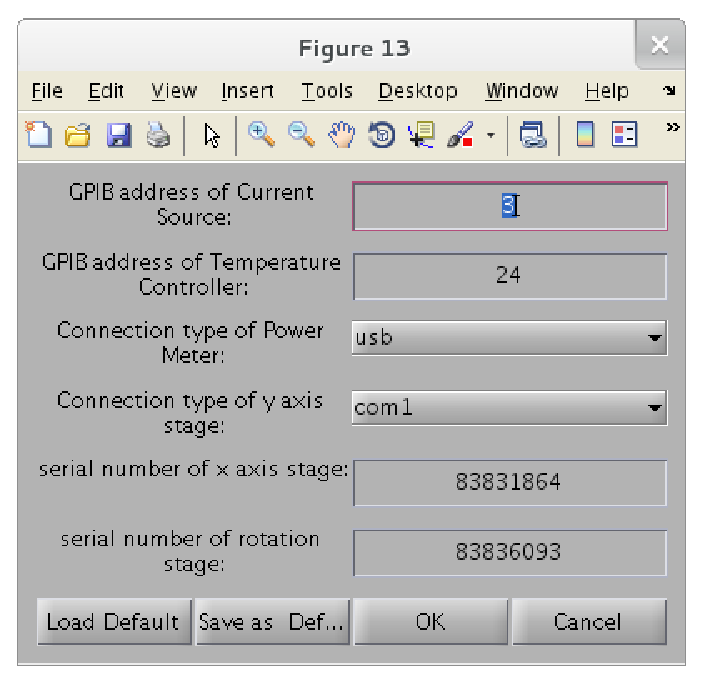
\includegraphics[width=0.5\textwidth]{./figs/setup.eps}
	\caption{FarfieldMeasurement Setup}
	\label{fig:setup}
\end{figure}

You will find four text edits, two popup menus and four buttons in this window.
Most of these components are self-explained. The first two text edits ask for
the gpib addresses of the current source and temperature controller since the
two instruments are controlled through GPIB interfaces. The following popup menu
asks for the connection type of the power meter. There are two options to
communicate our power meter. One is through USB and the other one is through
serial ports. If you want to use ``usb'' port, make sure ``usbdll.dll'' and
``NewpDll.h'' at the same directory as ``FarfieldMeasurement.m''. If you want to
use serial port, make sure you select the right ``com''
port(``com1'',``com2'',etc.) in the popup menu. The popup menu below asks for
the serial port(``com1'',``com2'',etc.) used to communicate the y axis linear
stage. The following two text edits ask for the serial number of x axis stage
and rotation stage. Both stages are controlled through Thorlabs controllers and
the serial numbers can be found on the controller. The ``Load Default'' button is used to load the default parameters to
overwrite the current parameters. The default setup is restored every time when
the program is called. The ``Save as Default'' button is used to save the
current parameters as the default setup. The ``OK'' button is used to accept the
current parameters and continue to next window. The ``Cancel'' button is used to
exit the program.

After the ``OK'' button is pressed to accept the parameters, the
Fig.~\ref{fig:main_window} will be shown.
\begin{figure}[htbp]
	\centering
	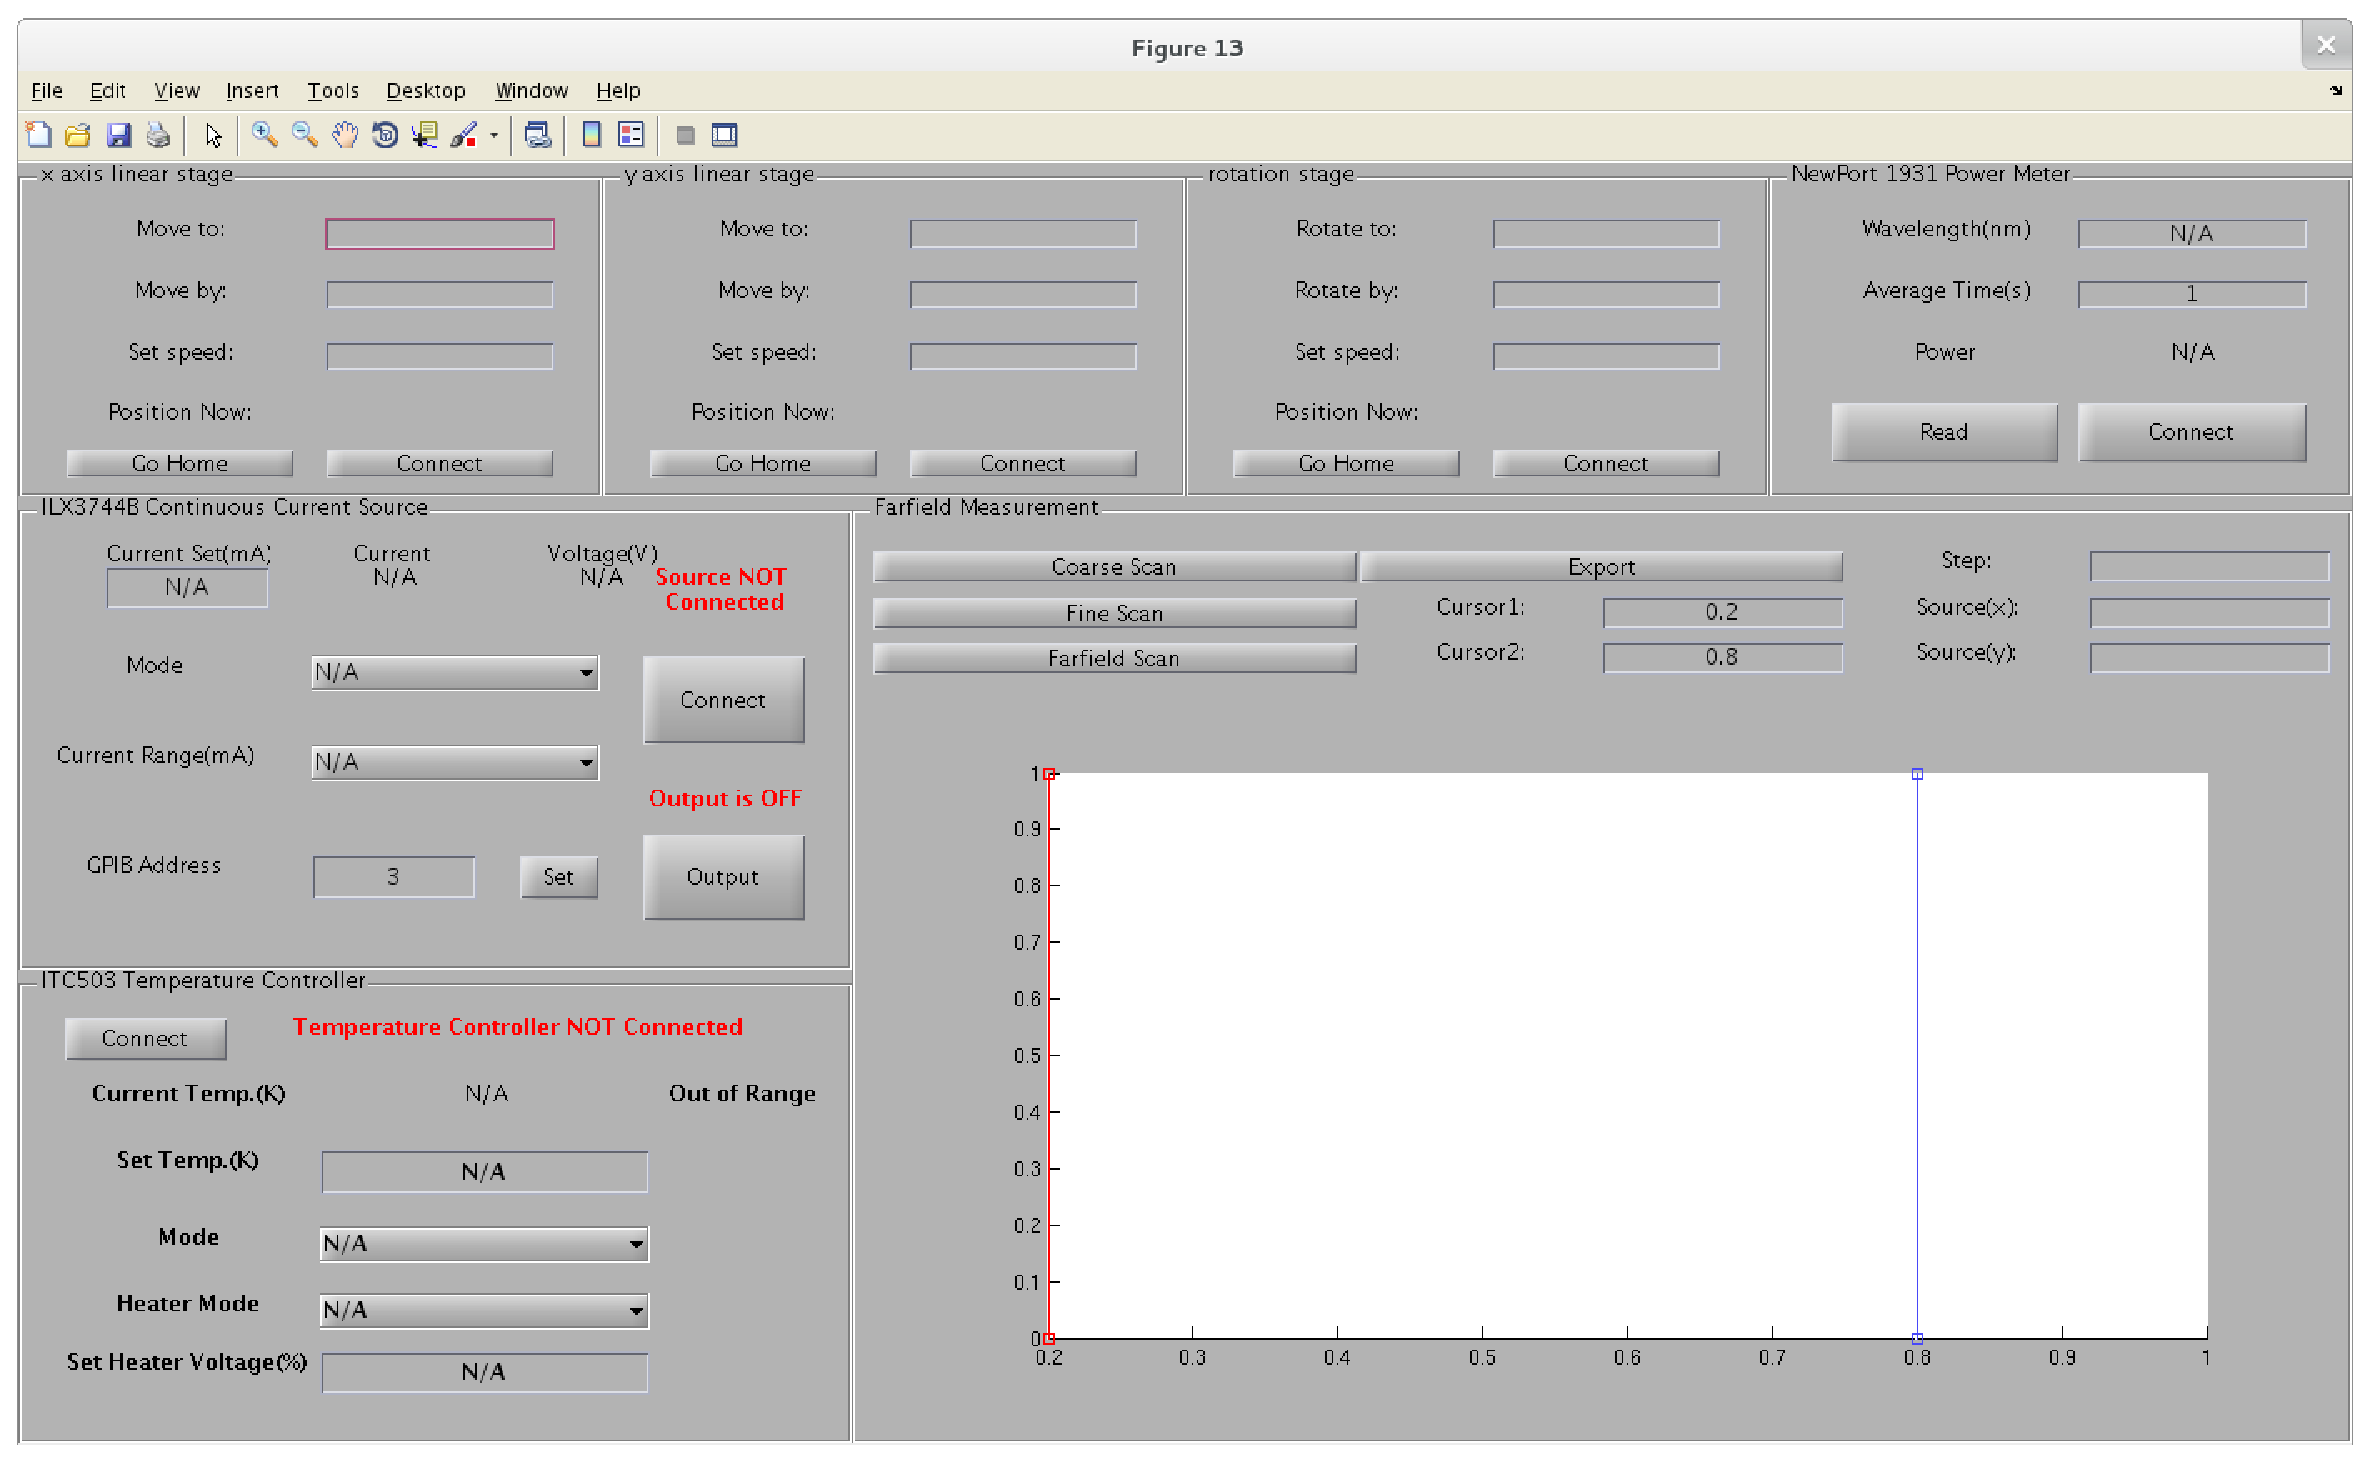
\includegraphics[width=0.9\textwidth]{./figs/main_window.eps}
	\caption{Main window}
	\label{fig:main_window}
\end{figure}

There are seven panels in this window. Each panel represents an equipment and is
plotted and controlled by the according class. The equipment name is shown in
the title region of each panel. In Fig.~\ref{fig:main_window}, you can find ``x
axis linear stage'', ``y axis linear stage'', ``rotation stage'', ``ILX3744B
Continuous Current Source'', ``ITC503 Temperature Controller'', ``NewPort 1931
Power Meter'' and ``Farfield Measurement'' in the title region. 

The ``x axis linear stage'', ``y axis linear stage'' and ``rotation stage''
panels have similar layout. There are three text edits, one is ``Move(Rotate)
to'', one is ``Move(Rotate) by'' and the other one is ``Set speed''. The
``Move(Rotate) to '' text edit can instruct the equipment to move(rotate) to a
absolute position. The ``Move(Rotate) by'' text edit can instruct the equipment
to move(rotate) by a relative position. The ``Set speed'' text edit can set the
speed of motion. There are also two buttons at the bottom of panels. The
``connect'' button will try to establish communication to the equipments. The
``Go Home'' button will instruct the equipment to go back to home position. The
``Position Now'' text shows the current position and will be refreshed
periodically. One note about the stages: make sure you are not moving the stage
beyond the range of stages and nothing is in the way of stages. One more note
about home position of the rotation stage: the home position of rotation stage
is stored when the stage is turned on. So if you want to set the home position
at a particular position, you should first turn the stage to the wanted
position, then turn off and on the rotation stage. The home position of the
other linear stages will be the zero position.

In the ``ILX3744B Continuous Current Source'' panel, the first text edit called
``Current Set'' is to set the output current. You should press ``enter'' button in
keyboard after the value is entered in this text edit to send the value to the
current source. The following two texts(``Current Output(mA)'', ``Voltage(V)'') show
the current and voltage information. These values will be updated periodically
when the communication is established. The red text ``Source NOT Connected'' shows
the connection status and it will change to green text ``Source Connected'' after
the connection is established. The button below is used to connect to the
current source. After clicked, if the connection is established, the text on the
button will change to ``Disconnect'' and used to disconnect the current source.
The red text ``Output is OFF'' shows the status of output enable. If the current
output is enabled by clicking the ``Output'' button below, the red text will
change to green text ``Output is ON''. There are two popup menus in this panel,
one is for the operation mode of current source and the other one is to set the
current range of current source. You can choose the proper one for your
measurement.

In the ``ITC503 Temperature Controller'' panel, the ``Connect'' button and red text
have the same function as mentioned above. The text bar below is used to show
the current temperature of the sensor which will be refreshed periodically when
connected. The text ``Out of Range'' shows the state of temperature stability.
Once the temperature is within 0.1K away from the set temperature, it will show
``Stable''. The text edit below is used to set temperature. You should press
``enter'' to confirm the set temperature. The ``Mode'' popup menu is used to show
the operation mode of the temperature controller. This parameter is to set how
you can operate the controller (remote or local) and whether to lock the front
panel of the controller (locked or unlocked). To have our gui remote controller
work, this has to be set as ``Remote\&Locked''. The popup menu below is used to
set the operation mode of heater and gas control. Since we don't have a gas
controller, the only thing that matters to us is the heater mode(Manual or
Auto). If the heater mode is set to be manual, the heater voltage below will be
used to set the heater power level. 

In the ``NewPort 1931 Power Meter'' panel, the ``Wavelength(nm)'' text edit shows
and sets the wavelength of the power meter. Once the power meter is connected by
clicking the ``Connect'' button, this text edit will be updated by the current
wavelength set in the power meter. You can enter your wavelength in this text
edit and press ``enter'' to confirm. The ``Average Time(s)'' text edit below is to
set how many seconds you want to average the measurement results. Once you
require the average power of the power meter, this is the time that the meter
used to average the results. The ``Power'' text below shows the instant power
level read from power meter periodically. The ``Read'' button is used to update
the power read instantly after pressing this button. 

In the ``Farfield Measurement'' panel, there are three subprograms called
``Coarse Scan'', ``Fine Scan'' and ``Farfield Scan''. To use coarse scan
subprogram, y axis linear stage should be first set at home position and then
the subprogram will instruct the y axis linear stage to move at a slow speed and
record the power read at a fixed time period. The result will be shown in the
below axes. The fine scan subprogram will instruct the y axis linear stage to
move from ``Cursor1'' position to ``Cursor2'' position by a step defined by
``Step''. You can set the cursor position by inputing the value in the
``Cursor1'' and ``Cursor2'' text edits. The farfield scan subprogram will scan
from ``Cursor1'' position to ``Cursor2'' position by a step defined by ``Step''
and then convert the position scale to angle scale based on the ``Source(x)''
and ``Source(y)'' values. The figure in the axes can be exported to an
independent figure and saved on your own. 

\end{document}

